\chapter{Principles of Germanium Detectors}
The phase of the detector medium plays an important role in radiation detection.
Gases, liquids, and solids are often used in scintillation detectors and can have huge detector volumes.
However, as shown above, some radiation can pass through these detectors due to gas and liquids having a low density and radiation such as gamma rays being quite penetrating.
Solids can be hundreds or thousands times more dense than gas and thus can have smaller detector volume to detect equivalent energy.
The problem is that even solid scintillation counters have poor energy resolution due to the small number of information carriers.
This is due to the fact that and incoming particle must go from radiation to light to electric signal which has extra steps where data can be lost and statistical fluctuations on small numbers create a limit to the energy resolution.
In order to reduce the statistical limit it is necessary to increase the number of information carriers.
Semiconductor detectors provide increased energy resolution due to more information carriers in terms of electron-hole pairs where the motion of these pairs in an applied electric field generates the electric signal.
Other advantages of semi conductor detectors are: compact size, relatively fast timing characteristics, and variable effective thickness based on application.
The two types of semiconductors most widely used are silicon and germanium.
Silicon is used primarily for charged particle spectroscopy while germanium is more widely used in gamma-ray spectroscopy.

\section{semiconductor diode detectors} 

The band structure of semiconductors is what makes them useful as radiation detectors in comparison to other metals or insulators
In a semiconductor, the valence band is made up of the electrons in the outer shell which are bound to specific lattice sites in the crystal.
In germanium they are covalent bonds that make up the interatomic forces within the crystal.
Above the valence band in terms of energy is the conduction band.
\begin{figure}[htpb]
\centering
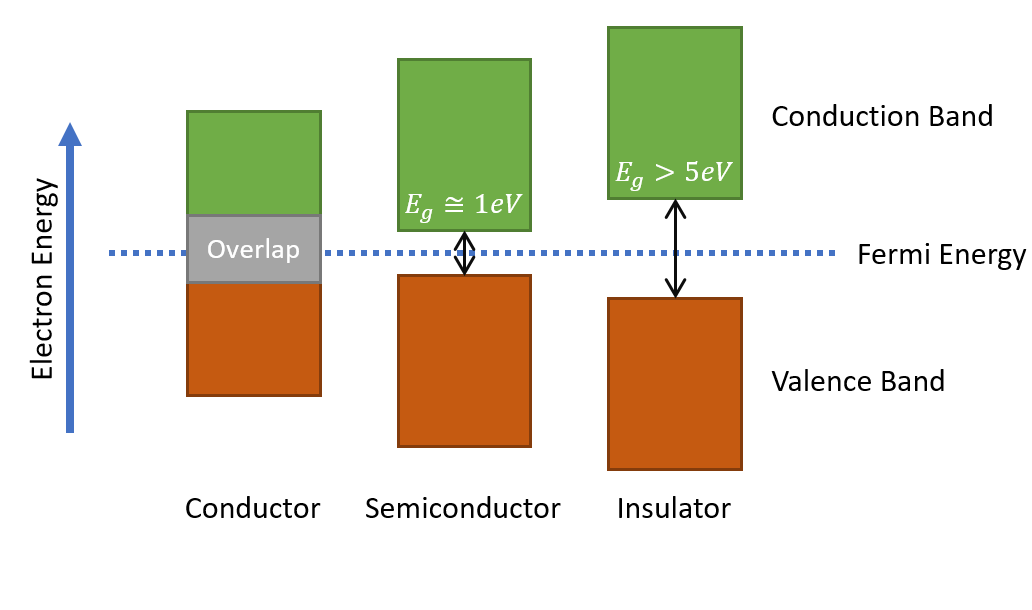
\includegraphics[width=0.9\textwidth]{bandgap}
\caption{Bandgap structures for different material types}
\label{fig:bandgap}
\end{figure}
The conduction and valence bands are separated by a bandgap which is specific to the material type.
The number of electrons inside the crystal just fills the valence band.
If the bandgap is small enough, electrons can sometimes have enough thermal energy to jump to the conduction band.
This energy comes from the crystal and electrons sharing thermal energy at temperatures above absolute zero.
The electron moving to the conduction band leaves behind an empty spot in the valence band which is called a hole.
If an electric field is applied to the crystal, the electron in the conduction band will drift parallel to the field in the opposite direction.
The hole is also acted upon by the field and will be forced to drift in the direction of the field.

All materials have some impurities that affect the crystal structure and can take the place of germanium atoms.
Some of them have electrons in the outer shells that exceed the amount required by the crystal lattice (4) and are thus weakly bonded.
It will not leave a hole behind when it is moved to the conduction band.
Impurities of this type are called donor impurities.
If a material is doped with atoms that have less electrons than required by the lattice, such as those from group III of the periodic table, there will be an extra hole available to be filled.  This is called an acceptor site.
\begin{figure}[htpb]
\centering
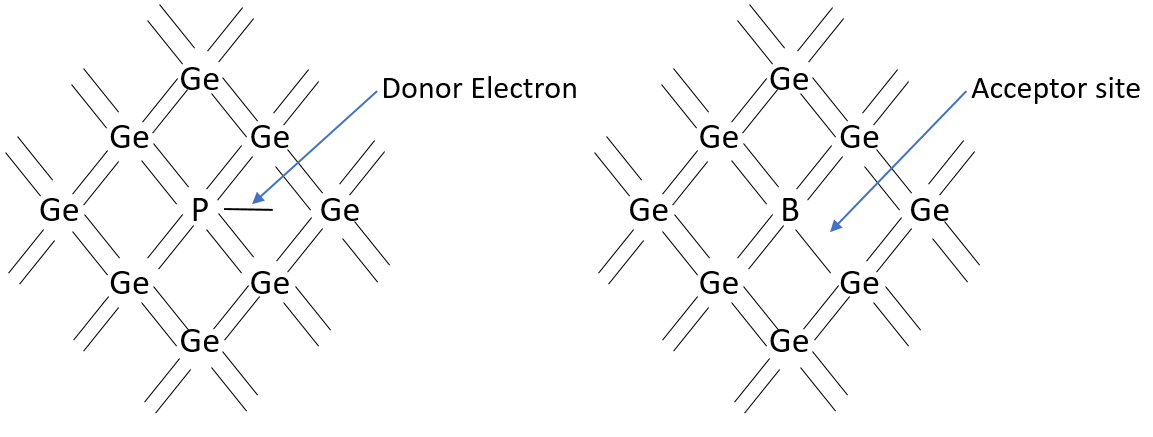
\includegraphics[width=\textwidth]{type}
\caption{Left: example of donor impurity configuration. Right: Example of acceptor impurity configuration}
\label{fig:type}
\end{figure}
An electron can fill an acceptor site where it will be left with a looser bond than the bulk of the crystal.
Whatever carrier is dominant determines the type of material.
Materials where electrons are the majority carrier, such as those doped with phosphorous, are called n-type semiconductors.
When the holes are the dominant information carrier, such as germanium doped with boron, the material is called p-type.

The energy required to create one electron-hole pair is called the ionization energy $\epsilon$.
When a charged particle travels through a detector it creates an amount of electron-hole pairs along its path proportional to the the incident particle energy.
There are always an equal numbers of electrons and holes created during an interaction event which lasts a few picoseconds.
Both carriers need to be fully collected in order to get an accurate energy measurement.

For the semiconductor to be a detector, there needs to be a way of collecting the charge generated by an event.
A typical event that deposits 1 MeV of energy in germanium will generate around $3\times 10^{5}$ electron hole pairs.
If all were drifted with an electric field and collected, it would only generate a current pulse of around $10^{-6}$A.
There needs to be a sufficiently low and stable current through the detector, such that when electron hole pairs are created, the added current pulse can be measured.
Thus it is necessary to have some sort of carrier blocking electrodes.
This will limit the amount of injected charge and current flowing through the bulk of the detector and bring the leakage current to sufficiently low levels.
Leakage current of the system needs to be on the order of $10^{-9}$A in order to be sufficiently low to not interfere with the radiation induced pulse.

In order to have an electric field capable of drifting the electrons and holes at their maximum velocity, the detectors are usually biased to several thousand volts.
This applied voltage can be either negative or positive depending on the detector material type and desired setup.
Once voltage is applied, the electrons and holes will start to drift relative to the field.
For example, in an unbiased p-type planar detector, holes are the dominant free moving carrier.
As the detector is biased, the holes are pushed away from the relatively positive charged electrode.
At higher and higher voltages, the holes are pushed further away from the electrode leaving a region of fixed negatively charged ions.
This region is called the depleted region and it becomes larger the more voltage that is applied.
When the detector is fully depleted, the electrons and holes become relatively fixed and there is no free movement of charge in the detector.

Typical semiconductor diode detectors are able to precisely measure radiation of alpha and beta particles, but have too small of a depletion region to measure the far more penetrating gamma rays.
However, the advent of HPGe detectors allowed for detectors with large volumes to be fully depleted.
Germanium (Ge) is a chemical element and has an atomic number of 32.
It is lustrous and grey in appearance.
It is hard as well as extremely brittle.
Ge is in the carbon group and is classified as a metalloid.
Germanium is most commonly used as a semiconductor in transistors and other electronic devices, notable high-purity Germanium detectors.
Due to its particularly narrow band gap, it has become widely used for radiation detection. 

The working principle of a germanium detector starts with some form of radiation interacting with the germanium and depositing some or all of its energy.
The incoming particle will interact with germanium atoms and cause a certain amount valence electrons, proportional to the energy deposited, to be kicked up to the conduction band.
Due to germanium detectors being operated under high voltage, large electric fields cause the drift of these electron hole pairs to the detector contacts where they can be collected.
This collection of electrons results in an electronic pulse that is amplified, shaped, and finally read out by a computer in the form of an energy spectrum.
\begin{figure}[htpb]
\centering
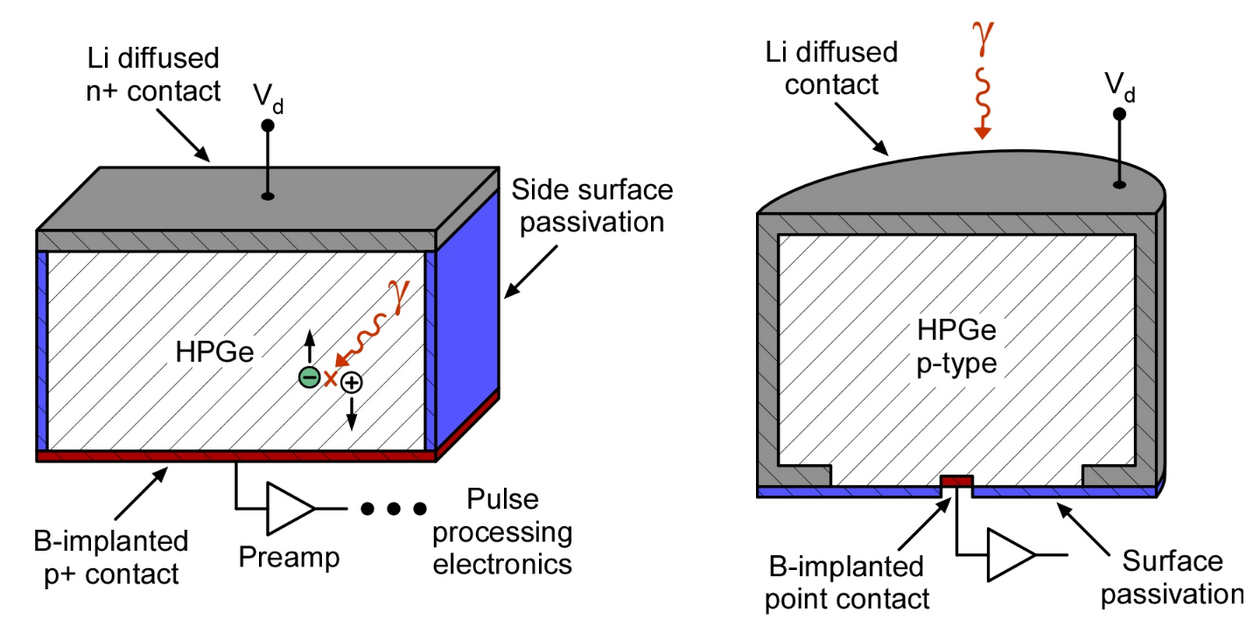
\includegraphics[width=\textwidth]{standard-ge}
\caption{Left: Planar HPGe detector with Li and B contacts. Right: Co-axial detector with Li and B contacts. Photo credit: Mark Amman}
\label{fig:standard-ge}
\end{figure}
Figure \ref{fig:standard-ge} shows a planar HPGe detector which is one of the simplest designs.
In order for the detector to work properly, it must be operated at a high voltage and it must also behave as a capacitor.
Behaving like a capacitor implies that there will be as little leakage current as possible, in other words that there will be no flow of current across the detector.
However, when an interaction happens, the electron hole pairs must be drifted and collected at the contacts.
This means that charge must be able to flow out of the detector but not back in.

It is the role of the detector contacts to provide this blocking of charge injection while facilitating readout of energy from an event.
The most common types of semiconductor contacts are impurity based or amorphous crystal.
For decades, the standard technology was to use a positive n+ lithium contact on one side and a negative p+ boron contact on the other.
The n-type lithium would block hole injection while the p-type boron would block electron injection on the other side due to the coulomb force.
The side surfaces must also be passivated in order to protect the inner material from becoming oxidized and created leakage current problems over time.

\begin{figure}[htpb]
\centering
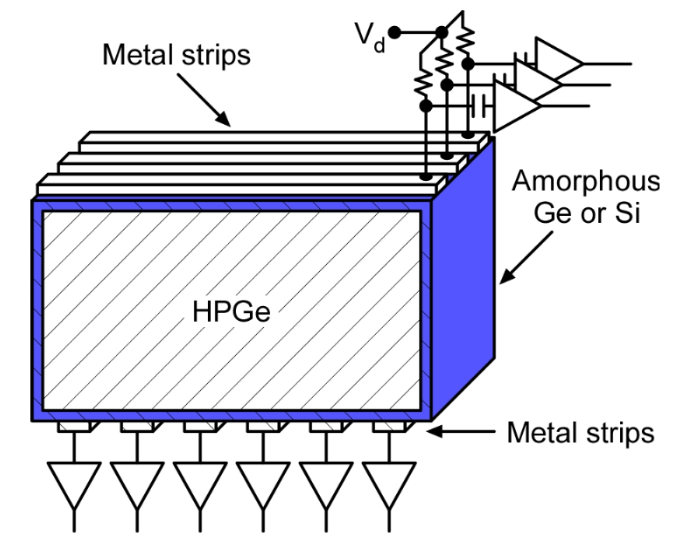
\includegraphics[width=0.6\textwidth]{age-strip}
\caption{HPGe strip detector with amorphous germanium contacts. Photo credit: Mark Amman}
\label{fig:age-strip}
\end{figure}
The problem with lithium diffusion and boron implantation comes when trying implement new designs such as segmented strip detectors.
The lithium diffuses a significant amount into the germanium while boron diffuses less but both leave a dead layer of the detector.
Thus a different type of contact is desired.
It should have a thin dead layer, not diffuse into the crystal, be mechanical robust, and have stable characteristics over time.
One contact method that fits this is an amorphous semiconductor contact such as amorphous germanium.

Amorphous germanium is special because it is bi-polar blocking meaning that it blocks the injection of both holes and electrons due to its effect on the barrier height of the bandgap.
Amorphous germanium can also be used to form the passivation layer on non contact surfaces.
On contact surfaces it provides charge injection barriers, blocking injection of charges from outside the detector, and on the sides it creates a passivation layer. 
Metal such as aluminum can then be deposited on top of the amorphous germanium to provide good electrical contact.

